In this chapter we will perform an analysis of the results obtained in the multiple experiments. The analysis will allow us to obtain information regarding the original algorithm and compare it with the improved algorithm. In the same way we will compare the results with those obtained by other metaheuristics.

\subsection{Comparison of results}
In order to be able to present a correct analysis, a summary table (Table~\ref{tblRpdComparison}) is made comparing the RPDs averages of each value of the groups of instances. These are presented in such a way that allows us to objectively observe the behavior of metaheuristics in the face of a given problem and a set of known data, as already mentioned in the beginning of this work.

In the summary table we can see that each record of the first column identifies the group of instances that was observed and measured. Each record in the second column refers to an average RPD for the BGBHS metaheuristic developed without any improvement. The following column shows the RPD averages for the BGBHS metaheuristic with the improvement associated with the variation of the $ p $ parameter in the Bernoulli trial. The following column refers to the averages of RPD per instance of the BH S-Shape algorithm and finally the BH Improved column refers to the RPD averages of this metaheuristic. Finally the last row, generalizes a total of all RPD for each algorithm tested, in order to make a single final analysis.

\begin{table}[H]
\centering
\begin{tabular}{|c|c|c|c|c|}
\hline
\multicolumn{1}{|l|}{\textbf{\begin{tabular}[c]{@{}l@{}}Instance\\ group\end{tabular}}} & \multicolumn{1}{l|}{\textbf{\begin{tabular}[c]{@{}l@{}}BGBHS \\ average RPD\end{tabular}}} & \multicolumn{1}{l|}{\textbf{\begin{tabular}[c]{@{}l@{}}BGBHS \\ Improved\\ average RPD\end{tabular}}} & \multicolumn{1}{l|}{\textbf{\begin{tabular}[c]{@{}l@{}}Black Hole\\ S-Shape\\ average RPD\end{tabular}}} & \multicolumn{1}{l|}{\textbf{\begin{tabular}[c]{@{}l@{}}Black Hole\\ Improved\\ average RPD\end{tabular}}} \\ \hline
4                                                                                       & 8.55                                                                                       & 1.12                                                                                                  & 7.66                                                                                                     & 2.28                                                                                                      \\ \hline
5                                                                                       & 20.71                                                                                      & 2.42                                                                                                  & 12.41                                                                                                    & 4.83                                                                                                      \\ \hline
6                                                                                       & 16.88                                                                                      & 1.53                                                                                                  & 13.80                                                                                                    & 7.74                                                                                                      \\ \hline
A                                                                                       & 15.61                                                                                      & 4.63                                                                                                  & 18.94                                                                                                    & 14.96                                                                                                     \\ \hline
B                                                                                       & 74.28                                                                                      & 6.14                                                                                                  & 24.89                                                                                                    & 18.79                                                                                                     \\ \hline
C                                                                                       & 24.25                                                                                      & 5.35                                                                                                  & 12.78                                                                                                    & 11.07                                                                                                     \\ \hline
D                                                                                       & 65.87                                                                                      & 11.42                                                                                                 & 22.78                                                                                                    & 14.20                                                                                                     \\ \hline
\multicolumn{1}{|l|}{\textbf{TOTAL}}                                                    & \textbf{32.31}                                                                             & \textbf{4.66}                                                                                         & \textbf{16.18}                                                                                           & \textbf{10.55}                                                                                            \\ \hline
\end{tabular}
\caption{RPD comparison}
\label{tblRpdComparison}
\end{table}


Regarding the group of instances 4, we can see that the worst result (8.55) in averages of RPD was for BGBHS in its version without improvements, whereas the best result (1.12) was for BGBHS with improvements. The best solution was followed closely by BH with improvements (2.28).\\

In the group of instances 5, a result very similar to 4 is produced. Where the worst RPD average result (20.71) was for BGBHS and the best (2.42) was for improved BGBHS, equally BH improved (4.83) closely follows the best average.\\

In the grouping of instances 6, the same pattern is followed as with the two cases previously reviewed, where the best RPD average (1.53) is for improved BGBHS and the worst result (16.88) is for traditional BGBHS. In this set of instances, there is a gap between improved BGBHS and BH improved by almost 6 points, although the same order is maintained when ranking from best to worst.\\

In the group of instances A, the tendency is broken, since the worst result in averages of RPD is for BH S-Shape (18.94) and the average between traditional BGBHS and improved BH is quite close with 0.61 difference. The best result continues to be for BGBHS with improvements (4.63).\\

For the group of instances B, we obtained the worst result in average RPD (74.28) for the metaheuristic BGBHS, even worse was the worst result of all sets of instances. Consistently the best result in averages of RPD was for BGBHS in its improved version. This time the gap between the best version of BGBHS and BH, distanced in 12.65, giving the advantage to BGBHS.\\

In the group of instances of C, we can see that the worst result in RPD averages obtained (24.25) was for BGBHS in its traditional version, while the best result in RPD averages (5.35) was for BGBHS in its improved version. They maintain a distance of 5.72 between the best average of BGBHS and the best of BH.\\

Finally in the group of instances D, the worst result in average RPD (65.87) was obtained by the metaheuristic BGBHS in its traditional version. The best result obtained in averages of RPD was obtained by BGBHS in its improved version. In this opportunity the distance between the best version of BGBHS and BH, decreased with respect to the group of previous instances, arriving at 2.78.\\

When we globally analyze the averages in RPD of all the results of each instance, Total row of the table \ ref {tblRpdComparison}, we can see that the trend analyzed in each group of instances is maintained.
The worst overall result is 32.31, which corresponds to the metaheuristic BGBHS in its classic version. On the other hand the best result on average RPD 4.66 corresponds to BGBHS in its improved version. When comparing the best overall RPD of BGBHS against BH, there is a difference of 6.49 in favor of Harmony Search.\\

Our results show that the improved version of BGBHS consistently beats BH in the two versions evaluated. On the other hand, the version of BGBHS in its classic version is beaten in all groups of instances by improved BH and in almost all BH S-Shape units except for instance group 6.\\

\begin{figure}[H]
\centering
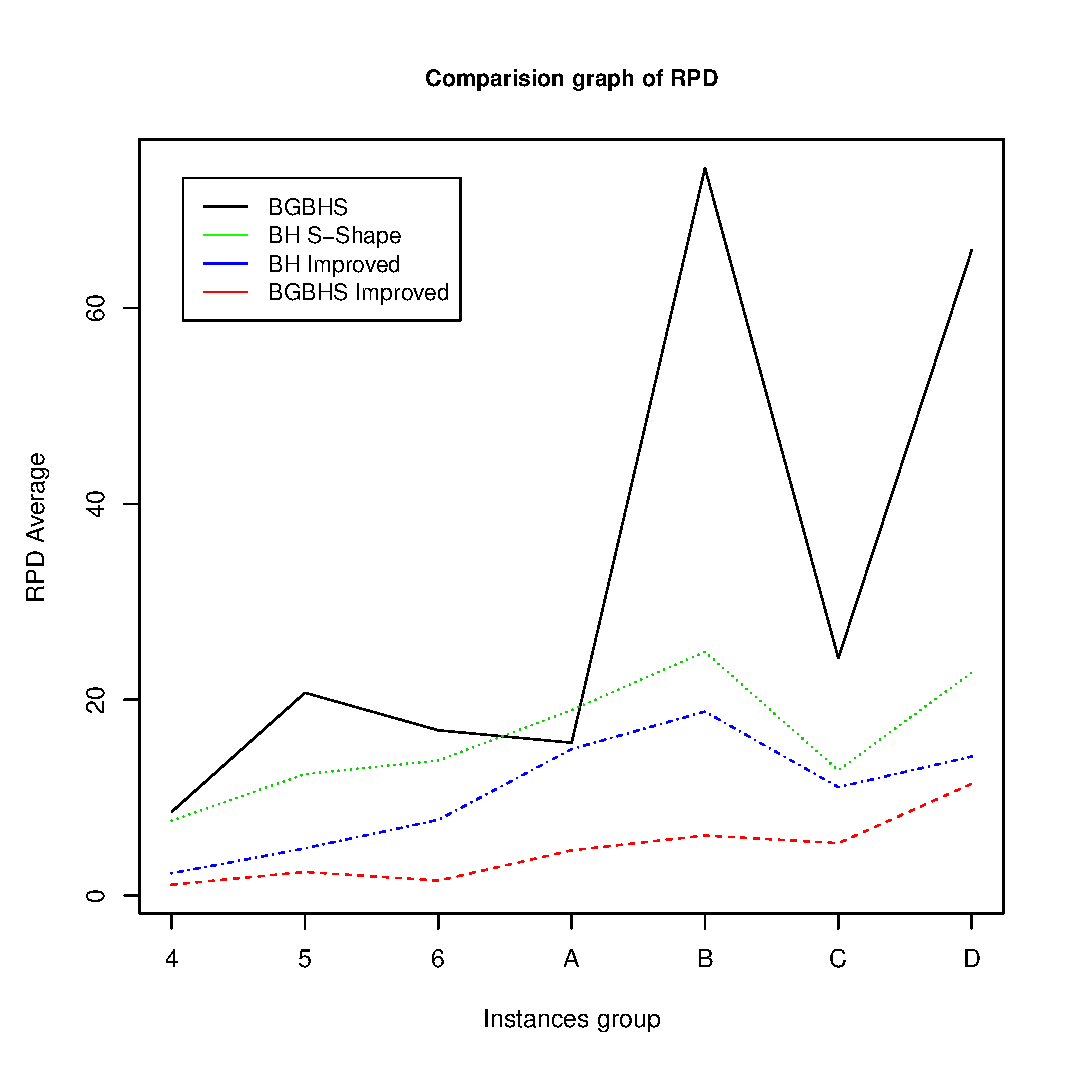
\includegraphics[scale=.55]{Conclusion/comparisionGraph.eps}
\caption{RPD average in each instance}
\label{fig:RPDAverage}
\end{figure}


